\chapter{Results and Discussion}
\label{ch:results}

%-------------------------------------------------------------------------------
% SECTION: Test Environment
%-------------------------------------------------------------------------------
\section{Test Environment}
Our test results were gathered on a 2011 MacBook Air \cite{bib:mba}: 1.8Ghz Intel Core i7 (Sandy Bridge i7-2677M) \cite{bib:sandy_bridge}, 4 GB 1333MHz DDR3 SDRAM, Intel HD 3000 Graphics (on CPU-die) with 384MB VRAM, and a solid-state (flash) hard disk. Our traditional architecture was represented by a 4.0GHz Intel i7-920 \cite{bib:i7-920}, with 6GB 1333MHz DDR3 SDRAM, ATI Radeon HD 5970 with 1GB VRAM \cite{bib:ati5870}, and a standard 7000RPM hard disk. For our software PBCB results, we forced OpenGL into a software-only mode.

%-------------------------------------------------------------------------------
% SECTION: Test Scene
%-------------------------------------------------------------------------------
\section{Test Scene}
Our test scene is an adapted Cornell Box. The Cornell Box was originally developed to quantify the difference between a Cornell renderer \cite{bib:cornell_box} and a real photograph of the same scene. However, due to its simple and elegant design, it has been adopted by the field of computer graphics as a standard for Global Illumination comparison (see \cite{bib:cornell_box_reference1}, \cite{bib:cornell_box_reference2}, \cite{bib:cornell_box_reference3}, \cite{bib:cornell_box_reference4}). Since its popularization circa 1985, it has become iconic and ubiquitous within the world of computer graphics.

This scene was chosen for its ability to showcase the subtleties of indirect illumination. The overhead area light casts clearly visible soft shadows around the cubes, and the color bleeding from the walls of the Cornell Box is prominently displayed in those shadows. Another demonstrative feature is that no direct light is cast on the ceiling; it is illuminated by purely indirect light.

Our Cornell Box is defined in a modified POV-Ray format \cite{bib:povray}, developed for the CSC 473 course at California Polytechnic State University, San Luis Obispo. It is comprised of 16 triangles, which make up the Cornell box, and 2 rotated and scaled cubes. This results in 14,000 surfels, following the algorithm in Section \ref{sec:surfel_generation}.

%-------------------------------------------------------------------------------
% SECTION: Analysis
%-------------------------------------------------------------------------------
\section{Analysis}
\label{sec:analysis}

\noindent Our analysis is threefold, based on the following metrics:
\begin{enumerate}
\item time to render one image
\item percieved image difference and quality
\item memory requirements
\end{enumerate}
\noindent We also discuss scalability in terms of geometric and shading complexity.

% ---- SUBSECTION: Speed ----
\subsection{Speed}
To analyze the speed of our GPU PBCB algorithm, we render our Cornell Box scene and compare it against both a Monte Carlo algorithm, and a forced software-mode of OpenGL. We demonstrate a 41.65x speedup over traditional Monte Carlo method, as well as a 3.12x speedup over the software-based renderer used in traditional PBCB, represented by an OpenGL software rasterizer. These results are collected in table \ref{tbl:renders}.

\begin{table}[h!]
   \centering
   \begin{tabular}{ | l | l | l | }
   \hline
   \textbf{Algorithm} & \textbf{Time (traditional)} & \textbf{Time (heterogenous)} \\ \hline
   16 MC samples & 525 sec & 565 sec \\ \hline
   32 MC samples & 790 sec & 862 sec \\ \hline
   64 MC samples & 1962 sec & 2137 sec \\ \hline
   128 MC samples & 3682 sec & 4063 sec \\ \hline
   256 MC samples & 7756 sec & 8205 sec \\ \hline
   Software PBCB & N/A & 615 sec \\ \hline
   GPU PBCB & 236 sec & 197 sec \\ \hline
   \end{tabular}
   \captionfonts
   \caption[Render times]{Render times for a 500x500 Cornell Box scene using our GPU PBCB algorithm compared against Monte Carlo with varying numbers of samples and traditional software-based PBCB. We include data for both traditional system architectures and heterogenous architectures where the GPU and CPU share their die.}
   \label{tbl:renders}
\end{table}

\begin{table}[h!]
   \centering
   \begin{tabular}{ | l | l | l | }
   \hline
   \textbf{Algorithm} & \textbf{Time Diff. (traditional)} & \textbf{Time Diff. (heterogenous)} \\ \hline
   16 MC samples & +123\% & +187\% \\ \hline
   32 MC samples & +235\% & +338\% \\ \hline
   64 MC samples & +731\% & +985\% \\ \hline
   128 MC samples & +1460\% & +1962\% \\ \hline
   256 MC samples & +3186\% & +4065\% \\ \hline
   Software PBCB & N/A & +212\% \\ \hline
   GPU PBCB & baseline & baseline \\ \hline
   \end{tabular}
   \captionfonts
   \caption[Render times speedup]{Differences in render times, as percent difference, for a 500x500 Cornell Box scene using GPU PBCB as a baseline compared against Monte Carlo with varying numbers of samples and traditional software-based PBCB. We include data for both traditional system architectures and heterogenous architectures where the GPU and CPU share their die.}
   \label{tbl:render_diffs}
\end{table}

As evidenced by our results from image comparisons in Section \ref{sec:img_quality}, we don't reach an acceptable noise level in the Monte Carlo algorithm until 256 samples. Therefore, we will frame our analysis of runtime by comparing our GPU PBCB algorithm against the 256 sample Monte Carlo render.

In this case we attain a 41.65x speedup on our heterogenous architecture system, and a 32.86x speedup on our traditional architecture system.

Another important feature of our work is the fact that we extend the basic PBCB implementation to leverage the GPU hardware to accelerate our algorithm. We were able to capture data for a software-based rasterizer by leveraging the ability to use a forced-software-mode OpenGL context. This was not possible on our traditional architecture as it only supported a software-based OpenGL 1.0 context, while we require OpenGL 2.0 features. However, we were able to force our heterogenous architecture system to use a software-based rendering context, and achieved a 3.12x speedup. We expect this speedup to be present on a traditional architecture system, but not to the same extent as it runs our algorithm 19.8\% slower in our tests.

% ---- SUBSECTION: Image Quality ----
\subsection{Image Quality}
\label{sec:img_quality}
In order to compare image quality, we must determine a baseline for comparison. For this we use our Monte Carlo algorithm. Specifically, we use a 256 samples for our Monte Carlo because we have found this to offer an acceptable level of noise. See figure \ref{fig:monte_carlo_noise} for noise comparisons between varying numbers of samples.

\begin{figure}
   \centering
   \subfloat[1 sample]{\label{fig:1mcs}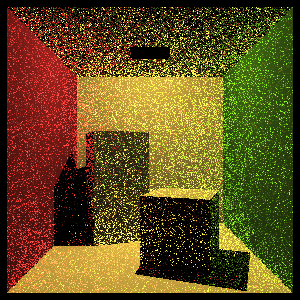
\includegraphics[width=50mm]{../img/cornell_simp_1mcs.png}}
   ~
   \subfloat[16 samples]{\label{fig:16mcs}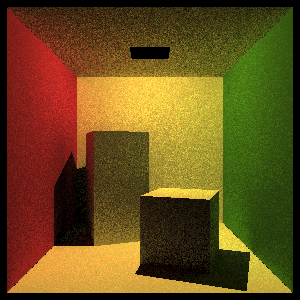
\includegraphics[width=50mm]{../img/cornell_simp_16mcs.png}}
   \\
   \subfloat[32 samples]{\label{fig:32mcs}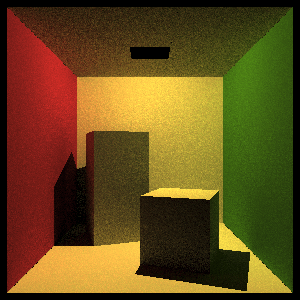
\includegraphics[width=50mm]{../img/cornell_simp_32mcs.png}}
   ~
   \subfloat[64 samples]{\label{fig:64mcs}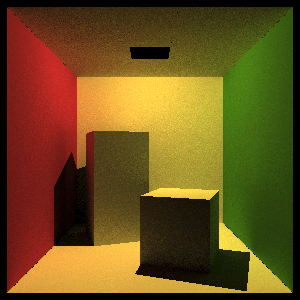
\includegraphics[width=50mm]{../img/cornell_simp_64mcs.png}}
   \\
   \subfloat[128 samples]{\label{fig:128mcs}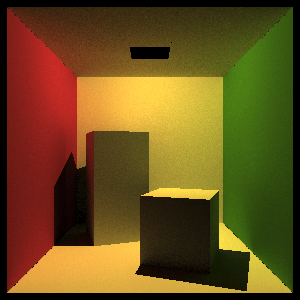
\includegraphics[width=50mm]{../img/cornell_simp_128mcs.png}}
   ~
   \subfloat[256 samples]{\label{fig:256mcs}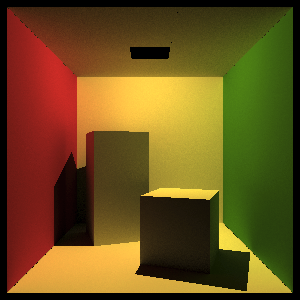
\includegraphics[width=50mm]{../img/cornell_simp_256mcs.png}}
   \captionfonts
   \caption[Monte Carlo noise]{Noise results from varying numbers of Monte Carlo samples in a Cornell Box with point light.}
   \label{fig:monte_carlo_noise}
\end{figure}

Using the mean absolute error image comparison algorithm implemented in ImageMagick compare \cite{bib:compare}, we can determine the difference between our 256 Monte Carlo baseline, and our GPU PBCB algorithm. The results are collected in table \ref{tbl:compare}.

\begin{table}[h!]
   \centering
   \begin{tabular}{ | l | l | }
   \hline
   \textbf{Algorithm} & \textbf{MAE} \\ \hline
   16 MC samples & 3.22\% \\ \hline
   32 MC samples & 2.78\% \\ \hline
   64 MC samples & 2.12\% \\ \hline
   128 MC samples & 1.83\% \\ \hline
   256 MC samples & 1.76\% \\ \hline
   GPU PBCB & baseline \\ \hline
   \end{tabular}
   \captionfonts
   \caption[Monte Carlo vs. GPU PBCB image comparison]{Image difference for the Cornell Box scene with the emissive geometry area light using our GPU PBCB algorithm compared against Monte Carlo with varying numbers of samples and traditional software-based PBCB. The listed values are mean absolute error computed as the average over each pixel pair and each color channel.}
   \label{tbl:compare}
\end{table}

The error percent values listed in table \ref{tbl:compare} show us that we have produced very similar images. This can be verified visually as well in figure \ref{fig:mc_gpu_pbcb_compare}. Our GPU PBCB algorithm produces renders that are most similar to the 256 sample Monte Carlo render, which is only 1.76% different on average. This makes intuitive sense as the noise in the lower sample rate renders causes a greater difference in appearance.

\begin{figure}
   \centering
   \subfloat[GPU PBCB]{\label{fig:256mcs}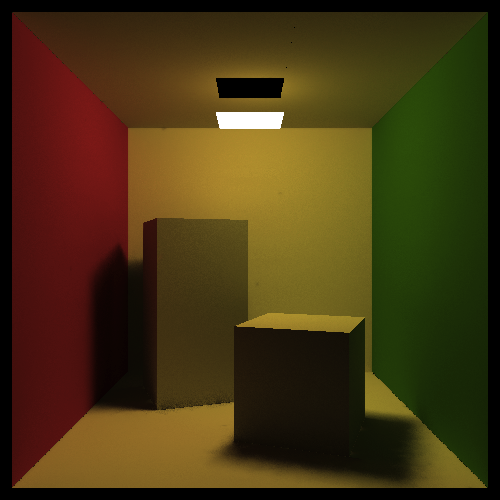
\includegraphics[width=70mm]{../img/cornell_simp_area_gpu_pbcb_3m_16s_696ms.png}}
   ~
   \subfloat[256 sample Monte Carlo]{\label{fig:gpu_pbcb}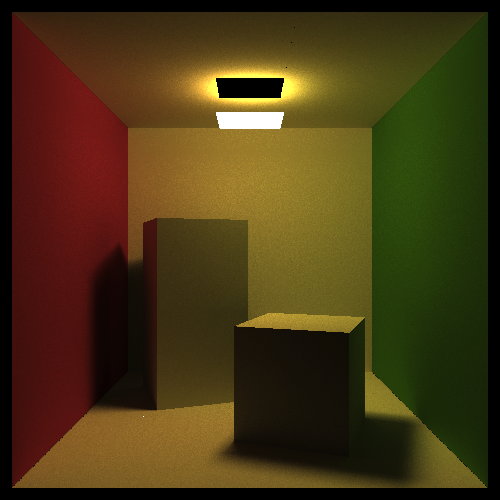
\includegraphics[width=70mm]{../img/cornell_simp_area_256mcs_2h_16m_44s_738ms.png}}
   \\
   \subfloat[Image Difference]{\label{fig:image_diff}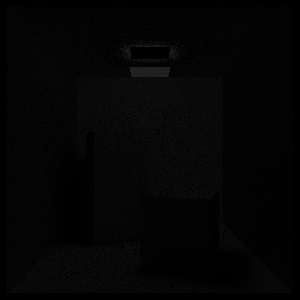
\includegraphics[width=70mm]{../img/area_error_mcs_surfs.png}}
   \captionfonts
   \caption[256 sample Monte Carlo vs. GPU PBCB]{Our Cornell Box rendered with both 256 sample Monte Carlo and our GPU PBCB algorithms. Included is an image produced by using the distance between two colors for all color channels per pixel.}
   \label{fig:mc_gpu_pbcb_compare}
\end{figure}

The error values are measures of mean absolute error. This is calculated by computing the difference between pairwise pixel’s color channels and averaging them over the entire set of pixels. For example, if our GPU PBCB algorithm produces a pixel with color values \textless0.45, 0.50, 0.45\textgreater, and the 256 sample Monte Carlo algorithm produces a pair pixel with values \textless0.1, 0.2, 0.1\textgreater, then the pairwise distance values are \textless0.35, 0.3, 0.35\textgreater, and the mean absolute error would be the average of these distances, i.e. 0.3333 or 33.33%.

Lastly, we have generated a difference image that was computed by using the absolute value of the difference between pairwise pixels in the two renders produced by our GPU PBCB algorithm and the 256 sample Monte Carlo render. This allows us to visualize the difference between renders.

It is important to note that the largest area of difference is the emissive geometry at the top of our Cornell Box. The difference is greatest here because of a limitation of our algorithm. Because we store direct illumination shaded surfels as triangles in a VBO on the GPU, we can only represent the color range from $\textless0,0,0\textgreater$ to \textless1,1,1\textgreater. This is actually a limitation of GPU hardware, as it only supports this range, clamping all color values outside of it. This is an issue for the emissive geometry, which has a greater than $\textless1,1,1\textgreater$ direct illumination value because it is emitting light. Our Monte Carlo implementation evaluates the direct illumination on demand without any clamping of values, and therefore receives the correct illumination values for the emissive geometry. However, the bright “halo” effect is not lost entirely in our GPU PBCB, so we find this acceptable.

% ---- SUBSECTION: Memory ----
\subsection{Memory}
Our memory usage was gathered by using the memusg script \cite{bib:memusg}. It polls the size reported by the unix utility ‘ps’ every 100 milliseconds and records the largest instantaneous memory usage.

When comparing our Monte Carlo and GPU PBCB algorithms in terms of memory, it is important to note that they share most of their code. The only difference is the indirect illumination computation. In this way, Monte Carlo is our baseline, and our GPU PBCB algorithm adds additional memory requirements. These are summarized in table \ref{tbl:memory}.

\begin{table}[h!]
   \centering
   \begin{tabular}{ | l | l | l | l | }
   \hline
   \textbf{Scene} & \textbf{MC Mem.} & \textbf{GPU PBCB Mem.} & \textbf {Diff.} \\ \hline
   1 object & 17.81 MB & 26.5 MB & +48.79\% \\ \hline
   2 objects & 17.81 MB & 26.6 MB & +49.35\% \\ \hline
   4 objects & 17.81 MB & 27.2 MB & +52.72\% \\ \hline
   8 objects & 17.82 MB & 28.5 MB & +59.93\% \\ \hline
   Cornell Box (18 Objects) & 17.83 MB & 31.8 MB & +78.35\% \\ \hline
   \end{tabular}
   \captionfonts
   \caption[Memory usage]{The memory usage for our Monte Carlo and GPU PBCB algorithms for varying numbers of geometric objects. Included is the percent increase in memory usage.}
   \label{tbl:memory}
\end{table}

\begin{figure}[h!]
    \centering
    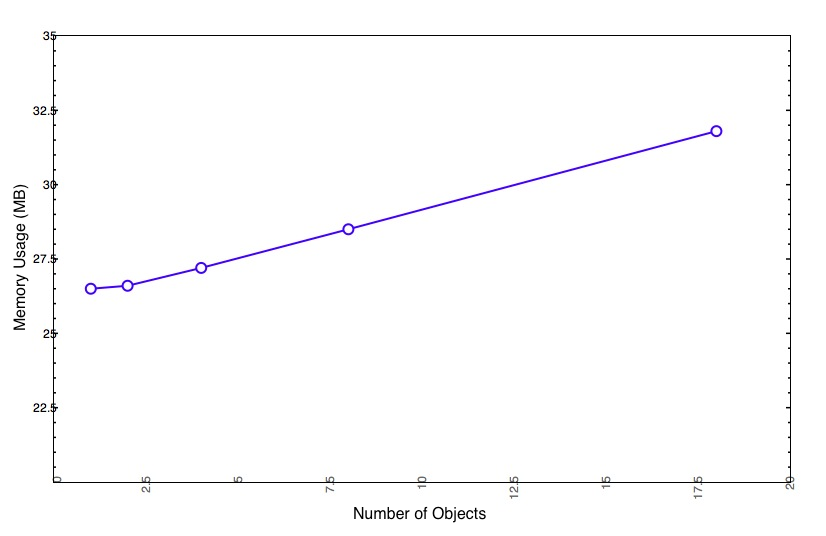
\includegraphics[width=150mm]{../img/memory.png}
    \caption[Memory Usage Graph]{Graph of our GPU PBCB memory usage for varying number of geometric objects in a scene.}
    \label{fig:memory_graph}
\end{figure}

The memory usage of our algorithm shows that we use a baseline of 48.79\% additional memory for one object. This baseline increases linearly with the number of objects in the scene (see figure \ref{fig:memory_graph}). This is due to the fact that each object adds a fixed number of additional surfels.

The baseline increase is due to the fact that our algorithm requires the OpenGL and helper libraries (e.g. GLUT), as well as the user-mode graphics driver. These are loaded in to our process’ address space and therefore increase its memory footprint.

It is also important to note that our Monte Carlo implementation increases its memory usage over time as well. However, it increases at a much slower rate than our GPU PBCB algorithm. This is because the Monte Carlo implementation only needs to store the base geometric object, but our GPU PBCB implementation stores that object as well as it’s associated surfels.

% ---- SUBSECTION: Scalability ----
\subsection{Scalability}
Scalability is the ability of our algorithm to scale to varying geometric complexity and image size. Because our algorithm supports only three types of geometry (i.e. triangle, sphere, and box), geometric complexity is a result of the number of surfels rasterized. To study this, we compare the render times for our Cornell Box with varying numbers of surfels generated. The results are collected in table \ref{tbl:geometry_scale}.

\begin{table}[h!]
   \centering
   \begin{tabular}{ | l | l | l | l | }
   \hline
   \textbf{Number of Surfels} & \textbf{Render Time} & \textbf{Mem. Usage} & \textbf{Surf. Gen. Time}\\ \hline
   9000 (500/obj.) & 199 sec & 31.8 MB & 16 sec \\ \hline
   18000 (1000/obj.) & 198 sec & 37.56 MB & 115 sec \\ \hline
   27000 (1500/obj.) & 184 sec & 43.03 MB & 380 sec \\ \hline
   36000 (2000/obj.) & 189 sec & 48.99 MB & 890 sec \\ \hline
   45000 (2500/obj.) & 192 sec & 54.44 MB & 1746 sec \\ \hline
   54000 (3000/obj.) & 202 sec & 59.90 MB & 2986 sec \\ \hline
   \end{tabular}
   \captionfonts
   \caption[Scalability: Geometric Complexity]{Comparison of GPU PBCB render times for varying numbers of surfels rasterized.}
   \label{tbl:geometry_scale}
\end{table}

Table \ref{tbl:geometry_scale} demonstrates that our render times are not affected by the number of surfels rasterized. This is due to the massive parallelism provided to us through the GPU. It can rasterize millions of triangles simultaneously, in parallel. For example, the ATI Radeon HD 5870 in our traditional architecture system can process 850 million polygons per second \cite{bib:ati5870}. However, our memory usage and surfel generation time are not constant.

Our memory usage scales linearly with the number of surfels required. This is expected and natural given that we’re simply generating and storing additional surfels. This can be seen in figure \ref{fig:surfel_memusg}.

Our surfel generation time is more interesting. Here we have an exponential growth curve for our render times based on how many surfels we generate per object. This is visualized in figure \ref{fig:surfel_gen_times_graph}. The reason for this is that our surfel generation algorithm uses an $O(n^{2})$ algorithm in order to determine the two closest points (see section \ref{sec:surfel_generation}).

\begin{table}[h!]
   \centering
   \begin{tabular}{ | l | l | l | }
   \hline
   \textbf{Image Size} & \textbf{Render Time} & \textbf{Mem. Usage} \\ \hline
   100x100 & 8 sec & 19.02 MB \\ \hline
   200x200 & 32 sec & 20.60 MB \\ \hline
   400x400 & 129 sec & 27.02 MB \\ \hline
   800x800 & 506 sec & 52.67 MB\\ \hline
   \end{tabular}
   \captionfonts
   \caption[Scalability: Image Size]{Comparison of GPU PBCB render times for varying image dimensions.}
   \label{tbl:img_scale}
\end{table}

\begin{figure}[h!]
    \centering
    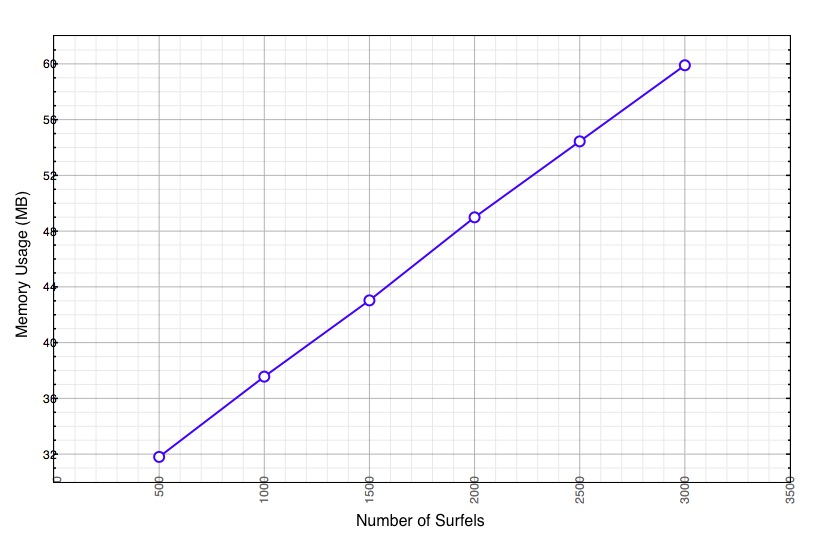
\includegraphics[width=150mm]{../img/surfel_memusg.png}
    \caption[Surfel Memory Usage Graph]{Graph of our GPU PBCB memory usage for varying number of surfels generated per object in our Cornell Box scene.}
    \label{fig:surfel_memusg}
\end{figure}

\begin{figure}[h!]
    \centering
    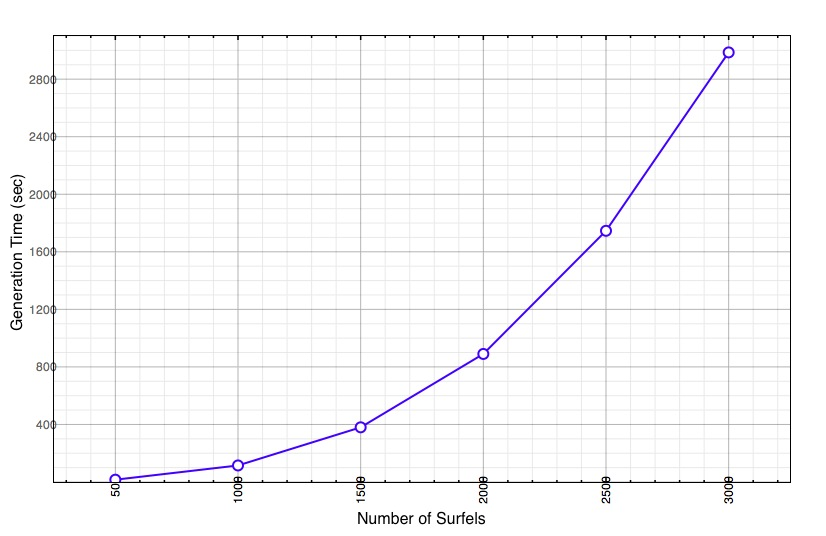
\includegraphics[width=150mm]{../img/surfel_gen_graph.png}
    \caption[Surfel Generation Time Graph]{Graph of our surfel generation times for varying number of surfels generated per object in our Cornell Box scene.}
    \label{fig:surfel_gen_times_graph}
\end{figure}

The other form of scalability we are interested in is how our algorithm scales to rendered image dimensions. The goal is linear scaling in each dimension, meaning that doubling the width and height should quadrouple the render time. The results are collected in table \ref{tbl:img_scale}, and clearly show that we do indeed scale linearly in both run time and memory usage.

%-------------------------------------------------------------------------------
% SECTION: Conclusions
%-------------------------------------------------------------------------------
\section{Conclusions}
In this thesis we have presented a GPU-accelerated implementation of the Point-Based Approximate Color Bleeding algorithm \cite{bib:christensen2008}. We have demonstrated a 41.65x speedup compared to 256 sample Monte Carlo ray-tracing, as well as a 3.12x speedup over PBCB using a software-based rasterizer.

We have also gathered data that compares traditional architecture systems with heterogenous architecture systems that place the GPU and CPU on the same die and share memory. We found that for our usage scenario, the heterogenous architecture achieves better performance despite comprising weaker specifications. However, this issue is not fully explored as our algorithm naively implements the cube-face rasterization. We believe it is possible to further explore rasterization batching and CPU-GPU parallelization in order to achieve even further performance gains, in which case the traditional may overtake the heterogenous architecture.

Lastly, we contribute a novel surfel generation algorithm that supports arbitrarily transformed geometry. This is important because proper coverage is a necessity to capture the proper shading in order to calculate indirect illumination as accurately as possible. And although our generation algorithm shows exponential growth as the number of surfels per object increases, we are pleased with the practical results in coverage we have obtained on transformed geometry.

%-------------------------------------------------------------------------------
% SECTION: Future Work
%-------------------------------------------------------------------------------
\section{Future Work}
\label{sec:future_work}

% ---- SUBSECTION: Persistent Surfel Storage ----
\subsection{Persistent Surfel Storage}
Currently, our algorithm stores the surfels in RAM, not a persistent file on the hard drive. This requires our renderer to re-generate the surfels for each render. One of the main benefits of PBCB in production is that it is possible for a scene to have surfels generated, persistently stored in a file, and loaded at render time to be reused. This amortizes the cost of the surfel generation process across all renders for the same scene.

In our renderer, the most effective way to implement persistent surfel storage would be to write the VBO array memory to a file as binary data, as opposed to storing it as text mesh-file format. In this way, a simple memory map operation would map the data directly into the VBO structure without any text parsing and processing whatsoever.

For our Cornell box scene, the surfel generation takes 16 seconds per render (see table \ref{tbl:geometry_scale}), which could be avoided with persistent surfel storage. And although the surfel generation is not included in our render runtime results, the feature would increase our overall render throughput.

% ---- SUBSECTION: Dynamic Surfel Surface Area Computation ----
\subsection{Dynamic Surfel Surface Area Computation}
Having a dynamic density for surfels would help to homogenize the surfel size throughout the scene. Our algorithm naively creates a user-provided number of surfels per geometric primitive: for triangles and spheres, exactly the specified number of surfels are generated, and for boxes, each face generates the specified number (i.e. specified value multiplied by six per box). This results in vaiable surfel sizes across the same geometric primitive at different scales. For example, the smaller triangles that compose the ceiling of our Cornell box, and the larger triangles that compose the walls, both generate 500 surfels. Because the primitives have different surface areas, the surfel density is variable, resulting in small surfels for the small triangles, and larger surfels for the large triangles.

Our proposed solution to this problem is to have a user-provided surfel density in the form of minimum distance. The current algorithm would be modified to continue decimating the random points until the specified minimum distance is met. Another way in which to achieve the same result, in perhaps a more intuitive manner, would be to have a user-provided surfel surface area. We would then solve for the minimum distance that would provide such a surface area, and use that, per the previously described algorithm modification.

Furthermore, it would behoove us to analyze the results of varying the surfel surface area on final render quality and speed, as well as surfel memory requirements. The tradeoffs to consider are that larger surface areas would result in fewer surfels, thus requiring less memory and reducing render times by requiring fewer triangle rasterizations. But smaller surfels would increase the sampling density of the scene's radiance information, resulting in more accurate indirect illumination values, and would decrease the surfel generation run-time by requiring fewer passes for the decimation step within our algorithm.

% ---- SUBSECTION: Rasterization Batching ----
\subsection{Rasterization Batching}
\label{sec:batching}
On more traditional CPU-GPU architectures, where the CPU and GPU must communicate via the PCI bus, care must be taken to avoid synchonous communication over the slow PCI bus \cite{bib:pci_press}. Due to the latency of GPU-to-GPU communication, it is in our best interest to batch as much of this communication as possible. In our algorithm, we raster each cube-face serially. This means that each 8x8 cube-face texture is rasterized, then copied from GPU to CPU memory, and processed. Therefore, each cube requires 5 data transfers (recall that the bottom of the cube is ignored). For heterogenous system architectures, like our test system, this transfer is instant as CPU and GPU share memory. However, this data transfer is the single most time-consuming task in our algorithm on more traditional CPU-GPU architectures. The communication from GPU to CPU can be reduced however.

We can accomplish fewer transfers by packing multiple cube-face textures into one single texture per cube. In this way, we amortize the cost of one GPU-to-CPU transfer over 5 textures. The algorithm for this technique would require one additional render pass, in which the 5 cube-face textures are texture-mapped to 5 screen-aligned quadrilaterals. This creates a texture atlas per cube that requires only one GPU-to-CPU transfer and can be indexed appropriately to extract the data for each cube-face.

This idea could be taken further: to batch the entire set of cubes, or some subset, as available memory and texture size dictates. Potentially, one thread could perform the standard direct illumination calculations via ray-tracing, while another thread rasterizes the surfel cloud onto cube-face textures, but stores them into one texture atlas for the entire scene. This is a very appealing idea to us because it would achieve great parallelism, as the CPU and GPU would be simultaneously leveraged to perform rendering tasks.

% ---- SUBSECTION: Parallelization ----
\subsection{Parallelization}
We believe the benefits of parallelization are apparent and will not discuss them further here. Suffice it to say that our algorithm can easily benefit from a model that divides primary pixels between multiple threads of control. In fact, this is precisely how our Monte Carlo ray-tracer accomplishes its parallelization. 

However, our code relies on the GLUT library \cite{bib:glut} to create and manipulate the OpenGL context. GLUT does not currently support mulithreaded applications. For this reason, although our implementation supports multithreaded rendering for Monte Carlo ray-tracing, it does not for our GPU Point-Based Color Bleeding algorithm. We have acquired our results in both cases with one thread only.
 
Any solution to this problem will involve porting the OpenGL code that leverages GLUT to another multithreading-friendly library. The Simple and Fast Multimedia Library is one such library that is freely available \cite{bib:sfml}. Preferably, the library would support one single context that is shared between all threads of control and serializes their access, but it could also be accomplished while using GLUT by wrapping the functionality and diligent use of IPC and thread synchronization. By sharing the context, the surfel data within the VBO memory does not need to be duplicated.

Another type of parallelization that many applications utilizing the GPU leverage is CPU-GPU parallelization. This is where concurrent work is performed on both hardware devices. That is to say: the CPU does not block on a GPU draw call. This can be accomplished via the process described in Section \ref{sec:batching}. Here, we can completely divide the rendering process into threads performing direct illumination via standard ray-tracing and threads performing indirect illumination via GPU PBCB. Because our two types of illumination have no interdependencies, two final images can be rendered, one with the direct illumination values, and the other with the indirect illumination values, and combined after both rendering passes are complete.

